\problemname{Jan Ersa}
Så här börjar en dikt av Gustaf Fröding:\\ 
{\em 
Jan Ersa ägde Nackabyn,\\
Per Persa ägde Backabyn \\
i By i Västra Ed. \\
Jan Ersa, \\
Per Persa, \\
de höllo aldrig fred.
}

När Jan Ersa och Per Persa, på äldre dagar, flyttade in till staden såg de till att de hamnade så långt
från varandra som möjligt. Skriv ett program som läser in information om gatorna i staden och som sedan
bestämmer mellan vilka två hus den kortaste vägen är som längst, och sedan svarar med längden av denna väg.

\begin{figure}[ht!]
\centering
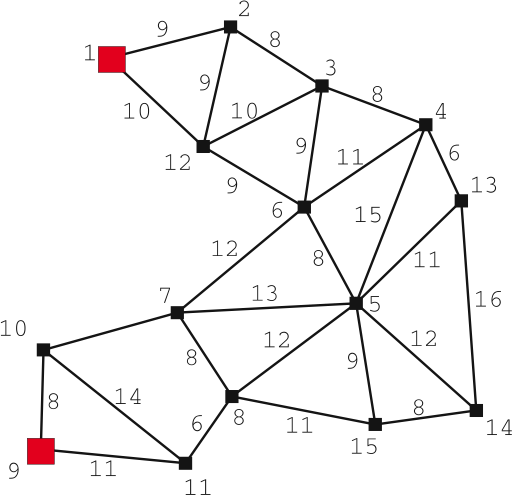
\includegraphics[width=0.4\textwidth]{janersa.png}
\caption{Kartan visar stadens alla hus och gator i exemplet. Vi ser också de röda husen där Jan Ersa och Per Persa numera bor. Dessa två hus (nr 1 och 9) är de hus i staden som ligger längst ifrån varandra (4900 meter).}
\label{overflow}
\end{figure}


\section*{Indata}
På första raden står ett tal $N$ ($2 \le N \le 100$), som anger antalet hus i staden. Husen är numrerade från $1$ till $N$. På nästa rad återfinns ett tal som anger antalet gator $V$, där $2 \le V \le 500$. Därefter följer $V$ rader med tre tal på varje rad: från hus nummer, till hus nummer och gatans längd (givet i 100-tals meter). I givna indata går det alltid att ta sig från vilket hus som helst till vilket annat hus som helst.

\section*{Utdata}
Skriv ut avståndet i meter mellan de två husen längst ifrån varandra.

\section*{Poängsättning}
Din lösning kommer att testas på en mängd testfallsgrupper.
För att få poäng för en grupp så måste du klara alla testfall i gruppen.

\noindent
\begin{tabular}{| l | l | p{12cm} |}
  \hline
  \textbf{Grupp} & \textbf{Poäng} & \textbf{Gränser} \\ \hline
  $1$    & $30$       & $N \leq 25$ \\ \hline
  $2$    & $70$       & Inga ytterligare begränsningar. \\ \hline
\end{tabular}
